\documentclass[12pt]{exam}
\usepackage[utf8]{inputenc}

\usepackage[margin=1in]{geometry}
\usepackage{amsmath,amssymb}
\usepackage{multicol}
\usepackage{mathrsfs}
\usepackage{amsmath}
\usepackage{graphicx}
\usepackage{tikz}
\usepackage{forest}
\tikzset{
  tree node/.style = {align=center, inner sep=0pt, font = \scriptsize},
  S/.style = {draw, circle, minimum size = 8mm, top color=white, bottom color=black!20},
  tree node label/.style={font=\scriptsize},
}
\forestset{
  declare toks={left branch prefix}{},
  declare toks={right branch prefix}{},
  declare toks={left branch suffix}{},
  declare toks={right branch suffix}{},
  tree node left label/.style={
    label=180:#1,
  },
  tree node right label/.style={
    label=0:#1,
  },
  maths branch labels/.style={
    branch label/.style={
      if n=1{
        edge label={node [left, midway] {$\forestoption{left branch prefix}##1\forestoption{left branch suffix}$}},
      }{
        edge label={node [right, midway] {$\forestoption{right branch prefix}##1\forestoption{right branch suffix}$}},
      }
    },
  },
  text branch labels/.style={
    branch label/.style={
      if n=1{
        edge label={node [left, midway] {\foresteoption{left branch prefix}##1\forestoption{left branch suffix}}},
      }{
        edge label={node [right, midway] {\forestoption{right branch prefix}##1\forestoption{right branch suffix}}},
      }
    },
  },
  text branch labels,
  set branch labels/.style n args=4{%
    left branch prefix={#1},
    left branch suffix={#2},
    right branch prefix={#3},
    right branch suffix={#4},
  },
  set maths branch labels/.style n args=4{
    maths branch labels,
    set branch labels={#1}{#2}{#3}{#4},
  },
  set text branch labels/.style n args=4{
    text branch labels,
    set branch labels={#1}{#2}{#3}{#4},
  },
  branch and bound/.style={
    /tikz/every label/.append style=tree node label,
    maths branch labels,
    for tree={
      tree node,
      S,
      math content,
      s sep'+=30mm,
      l sep'+=15mm,
      thick,
      edge+={thick},
    },
    before typesetting nodes={
      for tree={
        split option={content}{:}{tree node left label,content,tree node right label,branch label},
      },
    },
    where n children=0{
      tikz+={
        \draw [thick]  ([yshift=-10pt, xshift=-2.5pt].south west) -- ([yshift=-10pt, xshift=2.5pt].south east);
      }
    }{},
  },
}
\usepackage{tikz-qtree}
\usetikzlibrary{calc, shapes}

\newcommand{\class}{SA 405}
\newcommand{\term}{Fall 2018}
\newcommand{\examnum}{Final Exam}
\newcommand{\examdate}{Dec 14, 2018}
\newcommand{\timelimit}{180 Minutes}

\pagestyle{head}
\firstpageheader{}{}{}
\runningheader{\class}{\examnum\ - Page \thepage\ of \numpages}{\examdate}
\runningheadrule

%% Answer box macros
%% \answerbox{alignment}{width}{height}
\newcommand{\answerbox}[3]{%
  \fbox{%
    \begin{minipage}[#1]{#2}
      \hfill\vspace{#3}
    \end{minipage}
  }
}

%% \answerboxfull{alignment}{height}
\newcommand{\answerboxfull}[2]{%
  \answerbox{#1}{6.38in}{#2} 
}

%% \answerboxone{alignment}{height} -- for first-level bullet
\newcommand{\answerboxone}[2]{%
  \answerbox{#1}{6.0in}{#2} 
}

%% special boxes
\newcommand{\wordbox}{\answerbox{c}{1.2in}{.7cm}}
\newcommand{\catbox}{\answerbox{c}{.5in}{.7cm}}
\newcommand{\letterbox}{\answerbox{c}{.7cm}{.7cm}}



\begin{document}

\noindent
\begin{tabular*}{\textwidth}{l @{\extracolsep{\fill}} r @{\extracolsep{6pt}} r}
\textbf{\class} &&\textbf{\examnum}\\
\textbf{\term} &&\textbf{\examdate}\\
 && \\
 && \\
Midshipmen are persons of integrity.& \textbf{Name:} & \makebox[2.2in]{\hrulefill}\\\\
%\textbf{Time Limit: \timelimit} & Teaching Assistant & \makebox[2in]{\hrulefill}
\end{tabular*}

\noindent
\rule[2ex]{\textwidth}{2pt}

%This exam contains \numpages\ pages (including this cover page) and \numquestions\ questions.\\
%Total of points is \numpoints.

\begin{itemize}
\item Do {\bf not} write your name on each page, only write your name above.

\item No books or notes % or calculators
% that do symbolic manipulation (such as TI-89 or TI-92) 
 are allowed. %{\bf One} 8.5 by 11 inch formula/note sheet is allowed.

%\item You may use your calculator on this test.

\item Show all work clearly. (Little or no credit will be given for a numerical
answer without the correct accompanying work.
Partial credit is given where appropriate.) 

%\item If you need more space than is provided, use the back of the previous page. 

\item Please read the question carefully.
If you are not sure what a question is
asking, ask for clarification.

\item If you start over on a problem, please CLEARLY indicate what your final
  answer is, along with its accompanying work.

\item All formulations must have descriptions of any indices, parameters, and decision variables used. All constraints must be described. 
\end{itemize}


\begin{center}
Grade Table (for teacher use only)\\
\addpoints
\gradetable[v][questions]
\end{center}

\noindent
\rule[2ex]{\textwidth}{2pt}

\newpage %%%%%%%




\begin{questions}
\question Your regional manager at Dunder Mifflin, Michael Scott, has asked you to solve a Vehicle Routing Problem (VRP) to determine an optimal set of 3 paper-delivery routes for delivering paper to their 9 customers. He assumes that each route begins and ends at their warehouse in Scranton, PA. Mr. Scott also tells you that his goal is to minimize the total distance traveled among all vehicles. 

Each delivery route must be used, must visit at least two customers, and can transport no more than 425 cases of paper. Assuming that all distances are symmetrical, the table below gives the distances between the warehouse (WH) and each of the 9 customers.

\begin{table}[h]
\caption{Distances between the warehouse and all customers.}
\begin{center}
\begin{tabular}{|c|c|c|c|c|c|c|c|c|c|c|}
\hline
& WH &1&2&3&4&5&6&7&8&9\\ \hline
WH & - &10&12&13&40&25&16&37&23&19 \\ \hline
1& -  & - & 12 & 23 & 14 & 17 & 11 & 7 & 34 & 21 \\ \hline
2& -  & -  & - & 13 & 24 & 28 & 16 & 9 & 8 & 19 \\ \hline
3& -  & -  & -  & - & 24 & 26 & 14 & 13 & 12  & 5 \\ \hline
4& -  & -  & -  & -  & - & 5 & 37 & 17 & 8 & 9 \\ \hline
5&-  & -  & -  & -  & -  & - & 16 & 4 & 18 &  21 \\ \hline
6& -  & -  & -  &-  & -  & -  & - & 27 & 11 &  13 \\ \hline
7& -  & -  & -  & -  & -  & -  & -  & - & 18 & 9 \\ \hline
8& -  & -  & -  & -  &-  & -  &-  & -  & - & 19 \\ \hline
9& -  & -  & -  &-  & -  & -  & -  & -  & -   &- \\ \hline
\end{tabular}

\end{center}
\end{table}

\begin{table}[h]
\caption{Demand (in number of cases of paper) for each customer}
\begin{center}
\begin{tabular}{|c|c|}
\hline
Customer&Demand\\ \hline
1 & 20  \\ \hline
2 & 80  \\ \hline
3 & 90 \\ \hline
4 &  120\\ \hline
5 & 110 \\ \hline
6&  150\\ \hline
7& 100  \\ \hline
8& 75 \\ \hline
9& 85 \\ \hline
\end{tabular}

\end{center}
\end{table}

\vspace{.5cm}
Answer the following questions related to Michael Scott's request.
\begin{parts}
\part[10] Please provide an abbreviated \textbf{concrete} integer programming model for solving Mr. Scott's problem above. Clearly define your variables. Provide your objective function and all constraints required to solve Mr. Scott's problem. You can omit any subtour-elimination and route-splitting constraints in this formulation. \medskip \\
\answerboxone{c}{3in}\\
\part[5] You solve the problem again, and your solution thankfully contains no cycles. In this solution, vehicle 1 visits the sequence of customers $(1,6)$, vehicle 2 visits the sequence of customers $(2,4,5,7,8)$ and vehicle 3 visits the sequence of customers $(3,9)$. Is this solution feasible? If so, please provide a brief explanation why. If not, provide the appropriate set of constraints to eliminate this infeasible solution.\medskip \\
\answerboxone{c}{1.5in}
\part[5] Michael Scott comes to you to tell you that each vehicle can now only travel up to 80 miles along an entire delivery route. Compared to the original problem (without this travel distance maximum), do you expect the optimal objective function value for this new problem to increase, decrease, or remain the same? Give a brief explanation with your answer. \medskip \\
\answerboxone{c}{2in}

\end{parts}


\question There is currently an outbreak of the Ebola virus in the Democratic Republic of Congo (DRC). Once contracted with the Ebola virus, a person does not show any symptoms of the virus until two weeks after being infected. Given a limited budget, the World Health Organization (WHO) is looking to build temporary testing facilities that will be assigned to one or more cities to identify who has been infected in those cities. WHO's task is determine which of the three possible testing facilities should be built to maximize the total number of people tested for Ebola in the DRC.

\begin{itemize}

\item Sets:
\begin{itemize}
	\item[] $C:=$ Set of cities in the DRC.
	\item[] $F:=$ Set of possible facility locations in the DRC.
\end{itemize}

\item Parameters:
\begin{itemize}
\item[] $p_c:=$ The population of each city $c \in C$.
\item[] $p_f:=$ The maximum number of people facility $f \in F$ can test for Ebola.
\item[] $c_f:=$ The cost of building testing facility $f \in F$ in American dollars.
\item[] $B:=$ The budget of the WHO in American dollars.


\end{itemize}
\end{itemize}
\medskip

\begin{parts}
\part[4] Please provide all variables needed to model the WHO's problem as a mathematical programming model. \medskip
\\
\answerboxone{c}{1.5in}\\

\part[8] Using these variables, present an \textbf{abstract} mathematical programming model to maximize the total number of people tested for Ebola in the DRC without exceeding the WHO's budget. Clearly present an objective function and all appropriate constraints.\medskip
\\
\answerboxone{c}{4in}\\


\part[4] To cut costs, WHO has decided to change their objective. Instead of maximizing the total number of people tested, WHO has decided to minimize the total cost of building testing facilities as long as all people are tested for Ebola. Provide an updated objective function and provide any additional sets of constraint(s) required to appropriately model this problem. \medskip
\\
\answerboxone{c}{4in}\\
\part[4] To avoid cross-infection, the WHO has told you that you cannot simultaneously open facilities \#1 and \#3. Please provide the appropriate constraint(s) to model this restriction.\medskip \\
\answerboxone{c}{1in}\\

\end{parts}

\question[10] Given the graph $G$ in Figure \ref{primsfigure} below, execute Prim's algorithm to calculate a minimum spanning tree starting at vertex A. Show your steps in the table below. 

	\begin{figure}[h] 
	\label{primsfigure}
	\center
	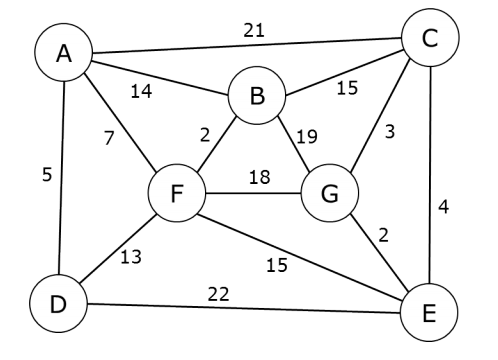
\includegraphics{prims_picture}
	\caption{Graph $G$}
	\end{figure}

As the algorithm iterates, provides all nodes in $S$, all edges in the cut-set $C_{S, \bar{S}}$, and the edges currently in the minimum spanning tree $T$. Break any ties by choosing the letter coming first in the alphabet. Finally, let $T$ contain the set of nodes forming the minimum spanning tree.
\begin{center}
\begin{tabular}{|c|c|c|c|}
\hline
Iteration \# & $\quad$ Set $S \quad$    & $\quad$ Cut-set $C_{S,\bar{S}}$ $\quad$	&$\quad$	Tree Edges $T$ $\quad$ \\ \hline
1 & &  &  \\ \hline
2 & & & \\ \hline
3 & & & \\ \hline
4 & & & \\ \hline
5 & & & \\ \hline
\end{tabular}
\end{center}
	
\question Given the graph $G_2$ in Figure \ref{bellmanfordfig} below, execute the Bellman-Ford algorithm to determine a shortest path from node $1$ to node $6$. 

\begin{figure}[h]
	\label{bellmanfordfig}
	\center
	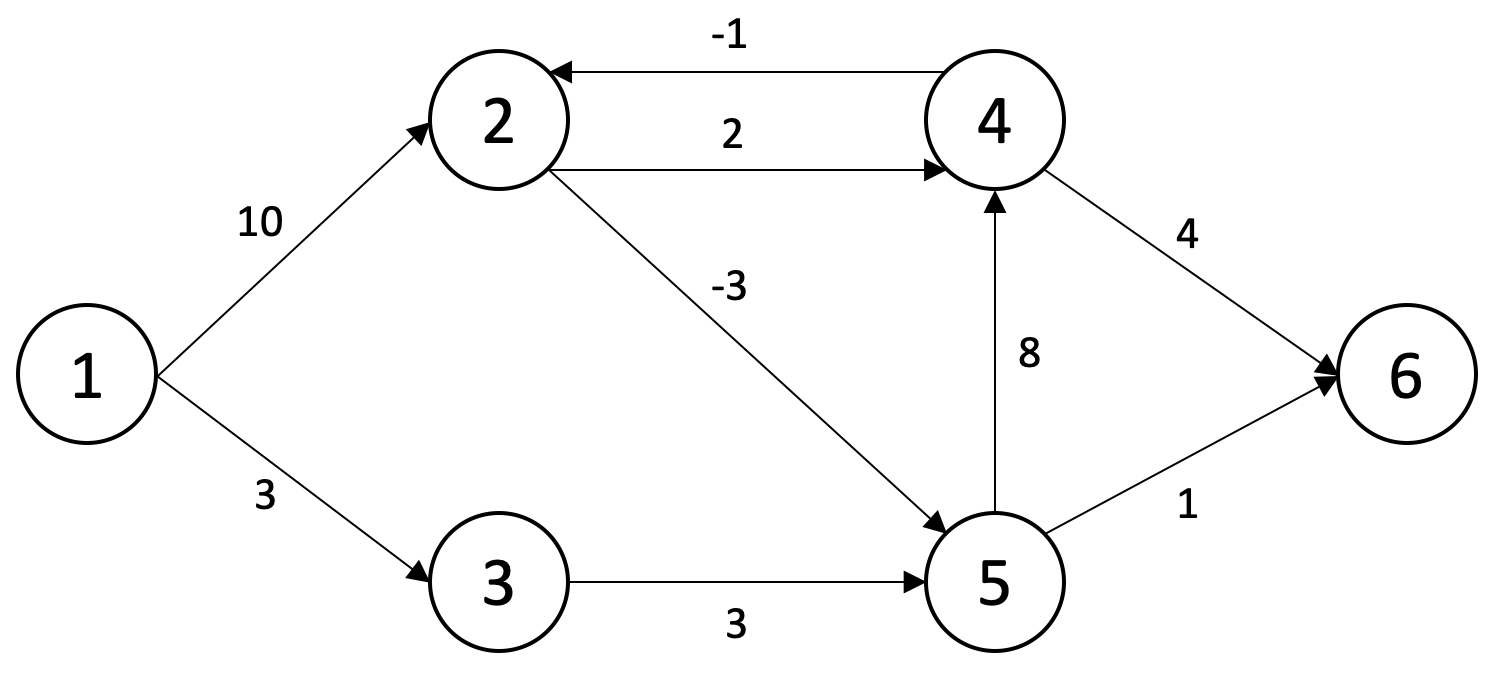
\includegraphics[width=8cm]{BellmanFordFigure}
	\caption{Graph $G_2$}
	\end{figure}
\begin{parts}
\part[8] Initialize each node with an appropriate distance label. As the algorithm iterates, cross out old distance labels and predecessors and update with the new values. Break any ties by choosing the minimum node label. 

\begin{center}
\begin{tabular}{|c|c|c|}
\hline
Vertex & \qquad Distance Label {\qquad}	& {\qquad}	Predecessor {\qquad} \\ \hline
A &  &  \\ \hline
B & & \\ \hline
C & & \\ \hline
D & & \\ \hline
E & & \\ \hline
F & & \\ \hline
G &  &  \\
\hline		
\end{tabular}
\end{center}

\part[2] Provide the final vector of distance labels $d$ and the final vector of predecessor labels $pred$.
\begin{itemize}
\item[] $d = \{ \ \ , \ \ , \ \  , \ \ , \ \ , \ \  \}$
\item[] $pred = \{ \ \ , \ \ , \ \  , \ \ , \ \ , \ \  \}$
\end{itemize}


\end{parts}
	
\end{questions}



\end{document}

